\documentclass[t,handout]{beamer}
\usepackage{verbatim}
\usepackage{xcolor}
\usepackage{multirow}
\usepackage{amssymb}
\usepackage{tikz}
\usepackage{hyperref}
\usetikzlibrary{positioning,fit}
%\usepackage{enumitem}
\usetheme{Warsaw}
\setbeamertemplate{navigation symbols}{}
\newcommand{\blue}[1]{{\color{blue} #1}}
\newcommand{\red}[1]{{\color{red} #1}}
\newcommand{\grn}[1]{{\color{green} #1}}
\newcommand{\bluRed}[2]{{\color{blue} #1}{\color{red} #2}}
\newcommand{\qtns}[0]{\begin{center} Questions? \end{center}}
\newcommand{\nl}[1]{\vspace{#1 em}}
\newcommand{\cntrImg}[2]{\begin{center}\includegraphics[scale=#2]{#1}\end{center}}
\newcommand{\defn}[1]{{\bf #1}}
\let\emptyset\varnothing
\newcommand{\SampS}[0]{$\mathcal{S}$}

\title{Math 3070, Applied Statistics}

\setlength{\abovedisplayskip}{0pt}
\setlength{\belowdisplayskip}{0pt}
\setlength{\abovedisplayshortskip}{0pt}
\setlength{\belowdisplayshortskip}{0pt}

\begin{document}
\begin{frame}[c]
    \begin{beamercolorbox}[rounded=true,wd=\textwidth,center]{title}
        \usebeamerfont{title}\inserttitle
    \end{beamercolorbox}
    \begin{center}
        Section 1\\
        \nl{0.5}
        November 18, 2019
    \end{center}
\end{frame}
\begin{frame}[c]{Lecture Outline, 11/18}
    Section 9.1 and 9.2
    \begin{itemize}
        \item Z-Test for the difference between two means.
        \item T-Test for the difference between two means.
    \end{itemize}
\end{frame}

\begin{frame}{Two-sample z Test}
    Suppose we are given two independent normal random samples:
    \begin{itemize}
    \item $X_1,\dots,X_m$
    \item $Y_1,\dots,Y_n$
    \end{itemize}
    \pause If we know the variances $\sigma_1^2$ and $\sigma_2^2$, we may use a \emph{two-sample z test} to test the null hypothesis $H_0: \mu_1-\mu_2 = \Delta_0$:
    
    \pause\begin{block}{}
    \begin{tabular}{c|c|c}
    Test Statistic & Alternative hypothesis & Rejection region \\ \hline
    \multirow{3}{*}{$\displaystyle Z=\frac{\overline X-\overline Y-\Delta_0}{\sqrt{\frac{\sigma_1^2}m+\frac{\sigma_2^2}n}}$} & $H_a: \mu_1-\mu_2>\Delta_0$ & $Z>z_{\alpha}$ \\
    & $H_a: \mu_1-\mu_2<\Delta_0$ & $Z<-z_{\alpha}$ \\
    & $H_a: \mu_1-\mu_2\neq\Delta_0$ & $|Z|>z_{\alpha/2}$\\
    \end{tabular}
    \end{block}
    
    \pause If $m$ and $n$ are large (say, $m>40$ and $n>40$), then we may use sample variances $S_1^2$ and $S_2^2$ in place of $\sigma_1^2$ and $\sigma_2^2$ and may drop the assumption that the distributions are normal.
    \end{frame}
    
    \begin{frame}{Example}
    \begin{block}{}
    A random sample of 20 specimens of cold-rolled steel had an average yield strength of 29.8 ksi. For a random sample of 25 two-sided galvanized steel specimens the average was 34.7 ksi. Assuming that the two yield-strength distributions are normal with $\sigma_1=4.0$ and $\sigma_2=5.0$, does the data provide significance evidence (at the $\alpha=.01$ level) for a difference between the mean yield strength of the two types of specimens?
    \end{block}
    
    \pause We want to test the null hypothesis $H_0: \mu_1-\mu_2=0$ against the alternative $H_a: \mu_1-\mu_2\neq 0$. \pause We calculate the test statistic:
    $$Z=\frac{\overline X-\overline Y-\Delta_0}{\sqrt{\frac{\sigma_1^2}m+\frac{\sigma_2^2}n}}
    \uncover<3->{= \frac{29.8-34.7-0}{\sqrt{\frac{(4.0)^2}{20}+\frac{(5.0)^2}{25}}}}
    \uncover<4->{=-3.65}$$
    
    \uncover<5->{The P-value for the test is $P(|Z|>3.65)=2\Phi(-3.65)=.00026$.}
    \uncover<6->{This provides strong evidence for a difference in the mean yield strengths of the two types of specimens.}
    \end{frame}
    
    \begin{frame}{z Confidence Interval for Difference of Two Means}
    Suppose we are given two independent normal random samples:
    \begin{itemize}
    \item $X_1,\dots,X_m$ from a $N(\mu_1,\sigma_1^2)$ distribution
    \item $Y_1,\dots,Y_n$ from a $N(\mu_2,\sigma_2^2)$ distribution
    \end{itemize}
    \pause Assume we know the variances $\sigma_1^2$ and $\sigma_2^2$.
    \pause \begin{block}{}
    A $100(1-\alpha)\%$ confidence interval for $\mu_1-\mu_2$ is given by
    $$\overline{X} - \overline{Y} \pm z_{\alpha/2}\sqrt{\frac{\sigma_1^2}m+\frac{\sigma_2^2}n}$$
    \end{block}
    \pause If $m$ and $n$ are large (say, $m>40$ and $n>40$), then we may use sample variances $S_1^2$ and $S_2^2$ in place of $\sigma_1^2$ and $\sigma_2^2$ and may drop the assumption that the distributions are normal.
    \end{frame}
    
    \begin{frame}{Example}
    \begin{block}{}
    A random sample of 20 specimens of cold-rolled steel had an average yield strength of 29.8 ksi. For a random sample of 25 two-sided galvanized steel specimens the average was 34.7 ksi. Assuming that the two yield-strength distributions are normal with $\sigma_1=4.0$ and $\sigma_2=5.0$, find a 95\% confidence interval for the difference in mean yield strength between the two types of specimens?
    \end{block}
    
    \pause
    \begin{align*}
    &\overline{X} - \overline{Y} \pm z_{\alpha/2}\sqrt{\frac{\sigma_1^2}m+\frac{\sigma_2^2}n}\\
    \uncover<3->{&= 29.8 - 34.7 \pm 1.96\sqrt{\frac{(4.0)^2}{20}+\frac{(5.0)^2}{25}}}\\
    \uncover<4->{&= -4.9 \pm  2.63}
    \end{align*}
    \end{frame}
    
    \begin{frame}{Two-Sample t Test (Welch's t Test)}
    Suppose we are given two independent normal random samples:
    \begin{itemize}
    \item $X_1,\dots,X_m$
    \item $Y_1,\dots,Y_n$
    \end{itemize}
    \pause If we don't know the variances $\sigma_1^2$ and $\sigma_2^2$, we may use a \emph{two-sample t test} to test the null hypothesis $H_0: \mu_1-\mu_2 = \Delta_0$:
    
    \begin{block}{}
    \begin{tabular}{c|c|c}
    Test Statistic & Alternative hypothesis & Rejection region \\ \hline
    \multirow{3}{*}{$\displaystyle T=\frac{\overline X-\overline Y-\Delta_0}{\sqrt{\frac{S_1^2}m+\frac{S_2^2}n}}$} & $H_a: \mu_1-\mu_2>\Delta_0$ & $T>t_{\alpha,\nu}$ \\
    & $H_a: \mu_1-\mu_2<\Delta_0$ & $T<-t_{\alpha,\nu}$ \\
    & $H_a: \mu_1-\mu_2\neq\Delta_0$ & $|T|>t_{\alpha/2,\nu}$\\
    \end{tabular}
    \end{block}
    
    \pause
    Here the degrees of freedom $\nu$ is estimated by
    $$\nu = \frac{\displaystyle \left(\frac{S_1^2}{m}+\frac{S_2^2}n\right)^2}{\displaystyle\frac{(S_1^2/m)^2}{m-1}+\frac{(S_2^2/n)^2}{n-1}}$$
    \end{frame}
    
    \begin{frame}{Example}
    The deterioration of many municipal pipeline networks across the country is a growing concern. One technology proposed for pipeline rehabilitation uses a flexible liner
    threaded through existing pipe. An article reported the following data on tensile strength (psi) of liner specimens both when a certain fusion process was used and when this process was not used:
    
    \begin{center}
    \begin{tabular}{l|p{9cm}}
    No fusion &
    2748
    3149
    2700
    2655
    2822
    2511
    3257
    3213
    3220
    2753
    \\ \hline
    Fusion &
    3027
    3356
    3359
    3297
    3125
    2910
    2889
    2902
    \end{tabular}
    \end{center}
    %pdf("ch9_dotplot.pdf",height=2,width=9);
    %par(mai=c(.5,1,0,0)+.05,omi=c(0,0,0,0)+.05,xpd=TRUE,las=1);
    %stripchart(list(nofus,fus),pch=19,at=1:2/3,ylim=c(0.25,.75),group.names=list("No fusion","Fusion"))
    %#stripchart(nofus,pch=19,xlim=c(2500,3400),add=TRUE,col="red",at=1)
    %dev.off();
    
    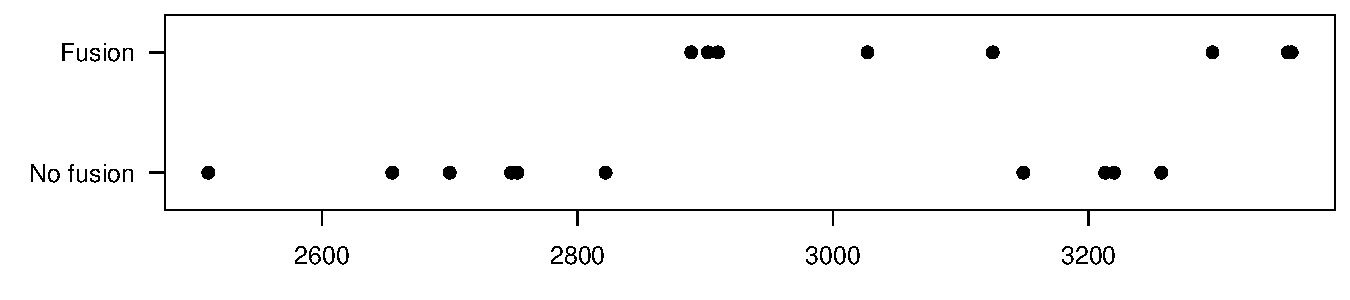
\includegraphics[scale=.5]{ch9_dotplot.pdf}
    \end{frame}
    
    \begin{frame}{Example}
    \begin{block}{}
    Does the data provide significant evidence for a difference in the mean tensile strength of the two types of specimens?
    \end{block}
    
    %\vspace{-.5cm}
    %\begin{center}
    %\begin{tabular}{l|p{9cm}}
    %No fusion &
    %2748
    %3149
    %2700
    %2655
    %2822
    %2511
    %3257
    %3213
    %3220
    %2753
    %\\ \hline
    %Fusion &
    %3027
    %3356
    %3359
    %3297
    %3125
    %2910
    %2889
    %2902
    %\end{tabular}
    %\end{center}
    %
    \pause We will test the null hypothesis $H_0: \mu_1-\mu_2=0$ against the alternative $H_a: \mu_1-\mu_2\neq 0$. 
    
    \pause The specimens with no fusion have $\overline X=2902.8$ and $S_1=277.3$, while those with fusion have $\overline Y=3108.1$ and $S_2=205.9$.
    
    \pause\begin{align*}
    T&=\frac{\overline X-\overline Y-\Delta_0}{\sqrt{\frac{S_1^2}m+\frac{S_2^2}n}}
    \uncover<5->{=\frac{2902.8-3108.1-0}{\sqrt{\frac{(277.3)^2}{10}+\frac{(205.9)^2}8}}}
    \uncover<6->{\approx -1.8} \\
    \uncover<7->{\nu &= \frac{\left( \frac{S_1^2}{m}+\frac{S_2^2}n\right)^2}{\frac{(S_1^2/m)^2}{m-1}+\frac{(S_2^2/n)^2}{n-1}} }
    \uncover<8->{= \frac{(7689.5+5299.3)^2}{\frac{(7689.5)^2}9+\frac{(5299.3)^2}7} }
    \uncover<9->{= 15.9 \approx 16}
    \end{align*}
    \uncover<10->{The P-value for the test is $$P(|T|>1.8)=2P(T>1.8)=2\cdot .045 =.090$$}
    \end{frame}
    
    \begin{frame}{t Confidence Interval for Difference of Two Means}
    Suppose we are given two independent normal random samples:
    \begin{itemize}
    \item $X_1,\dots,X_m$ from a $N(\mu_1,\sigma_1^2)$ distribution
    \item $Y_1,\dots,Y_n$ from a $N(\mu_2,\sigma_2^2)$ distribution
    \end{itemize}
    \pause Assume we \textit{do not} know the variances $\sigma_1^2$ and $\sigma_2^2$.
    \pause \begin{block}{}
    A $100(1-\alpha)\%$ confidence interval for $\mu_1-\mu_2$ is given by
    $$\overline{X} - \overline{Y} \pm t_{\alpha/2,\nu}\sqrt{\frac{S_1^2}m+\frac{S_2^2}n}$$
    \end{block}
    \pause Here, as before the degrees of freedom $\nu$ is estimated by
    $$\nu = \frac{\displaystyle \left(\frac{S_1^2}{m}+\frac{S_2^2}n\right)^2}{\displaystyle\frac{(S_1^2/m)^2}{m-1}+\frac{(S_2^2/n)^2}{n-1}}$$
    \end{frame}
    
    \begin{frame}{Example}
    \begin{block}{}
    Based on the pipeline liner data, find a 95\% confidence interval for the difference in mean tensile strength between the two types of specimens (no fusion vs. fusion).
    \end{block}
    \pause The specimens with no fusion had $\overline X=2902.8$ and $S_1=277.3$, while those with fusion had $\overline Y=3108.1$ and $S_2=205.9$. We calculated that the appropriate degrees of freedom was $\nu\approx 16$. \pause This leads to a critical value of $t_{.025,16}=2.120$. \pause A 95\% confidence interval for the difference $\mu_1-\mu_2$ is then given by
    \begin{align*}
    &\overline{X} - \overline{Y} \pm t_{\alpha/2,\nu}\sqrt{\frac{S_1^2}m+\frac{S_2^2}n} \\
    \uncover<5->{&= 2902.8-3108.1 \pm 2.120\sqrt{\frac{(277.3)^2}{10}+\frac{(205.9)^2}8}\\}
    \uncover<6->{&= -205.3 \pm  241.6}
    \end{align*}
    \end{frame}
    
    \begin{frame}{Problem}
    An article \footnote{``Trace Metals of South Indian River" (Envir.
    Studies, 1982: 62--66)} reports on a study in which six river locations were selected
    and the zinc concentration (mg/L) determined for both
    surface water and bottom water at each location:
    
    \begin{center}
    \begin{tabular}{l|cccccc}
    Location & 1 & 2 & 3 & 4 & 5 & 6 \\ \hline
    Bottom water &
    .430 & .266 & .567 & .531 & .707 & .716 \\ \hline
    Surface water &
    .415 & .238 & .390 & .410 & .605 & .609 \\ \hline
    %Difference &.015 & .028 & .177 & .121 & .102 & .107
    \end{tabular}
    \end{center}
    
    \pause \begin{block}{}
    Does the data provide significant evidence the mean zinc concentration in bottom water exceeds that of surface water?
    \end{block}
    
    \pause 
    \vspace{-.6cm}
    \begin{center}
    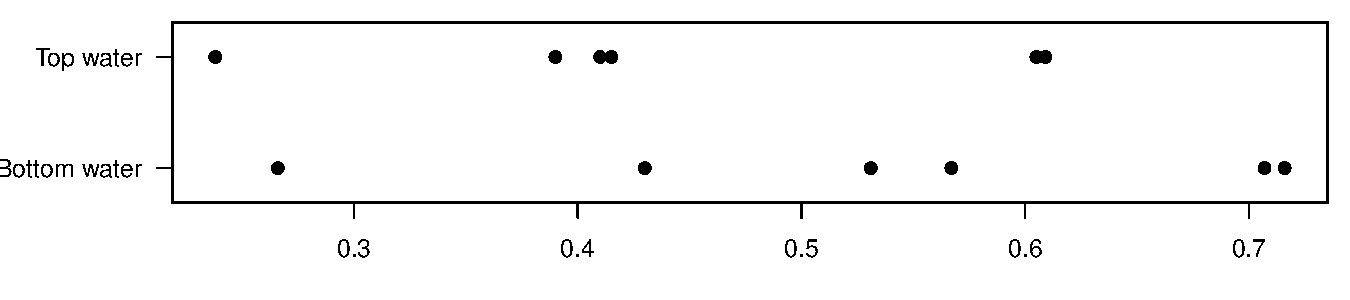
\includegraphics[scale=.5]{ch9_dotplot2.pdf}
    \end{center}
    %bot=scan(text=".430 .266 .567 .531 .707 .716");
    %top=scan(text=".415 .238 .390 .410 .605 .609");
    %pdf("ch9_dotplot2.pdf",height=2,width=9);
    %par(mai=c(.5,1,0,0)+.1,omi=c(0,0,0,0)+.05,xpd=TRUE,las=1);
    %stripchart(list(bot,top),pch=19,at=1:2/3,ylim=c(0.25,.75),group.names=list("Bottom water","Top water"))
    %dev.off();
    \end{frame}
    
    \begin{frame}{Problem}
    
    We want to test the null hypothesis $H_0: \mu_1-\mu_2=0$ against an alternative $H_0:\mu_1-\mu_2>0$ based on the data:
    
    \begin{center}
    \begin{tabular}{l|cccccc}
    Location & 1 & 2 & 3 & 4 & 5 & 6 \\ \hline
    Bottom water ($X_i$) &
    .430 & .266 & .567 & .531 & .707 & .716 \\ \hline
    Surface water ($Y_i$) &
    .415 & .238 & .390 & .410 & .605 & .609 \\ \hline
    %Difference &.015 & .028 & .177 & .121 & .102 & .107
    \end{tabular}
    \end{center}
    
    \pause It may seem natural to treat this as a two-sample problem: We could calculate $\overline X=.536$, $S_1=.171$, $\overline Y=.444$, and $S_2=.142$:
    \pause\begin{align*}
    T &= \frac{\overline X-\overline Y-\Delta_0}{\sqrt{\frac{S_1^2}m+\frac{S_2^2}n}}
    \uncover<4->{= \frac{.536-.444-0}{\sqrt{\frac{(.171)^2}6+\frac{(.142)^2}6}} }
    \uncover<5->{\approx 1.0\\ }
    \uncover<6->{\nu &= \left(\frac{S_1^2}{m}+\frac{S_2^2}n\right)^2 \div \left(\frac{(S_1^2/m)^2}{m-1}+\frac{(S_2^2/n)^2}{n-1}\right) }
    \uncover<7->{= 9.7 \approx 10 \\}
    \uncover<8->{P &= P(T>1.0) }
    \uncover<9->{= .170}
    \end{align*}
    \uncover<10->{However, this method would be \textit{incorrect} because the two samples are not independent of each other!}
    \end{frame}

\end{document}